\chapter{Motivation architecture}
\label{sec:motivation-architecture}

	This chapter presents the motivation and goal structure of the LAM team for this project. This motivation structure is also situated in the context of the Publications Office, this way providing a rationale for the initiative for modelling LAM data in the first place. 
		
	This motivation view helps address questions on why a stakeholder demand for certain capabilities is meaningful, model crucial drivers and root causes behind the demand, actual goals and related outcomes, as well as concrete requirements for further development. In short, it answers the crucial questions to WHOM, WHY and WHAT.
	
	We do not aim for an in depth coverage of the motivation architecture here: in the sense that it cannot be considered as a fully fledged decision-making tool for the management. The focus is to account for the context, stakeholders and their drivers and interests.
	
	\section{Prototypical motivation structure}
	\label{sec:how-to-motivation}		
	
	The structure of motivations, in ArchiMate, is organised hierarchically in several layers. For simplicity, we have chosen to use the top four layers: \textit{stakeholders, drivers, assessments and goals}; leaving out the \textit{outcomes}, \textit{principles} and \textit{requirements}. \mbox{Figure \ref{fig:morivation-structure}} depicts the organisation of the motivation architecture. The structure starts at the top with enumerating the stakeholders, who can be individuals, teams or organisations that represent their interests in the effects of \mbox{the architecture \citep{archimate3.1}}. 
	
	\begin{figure}[h]
		\centering
		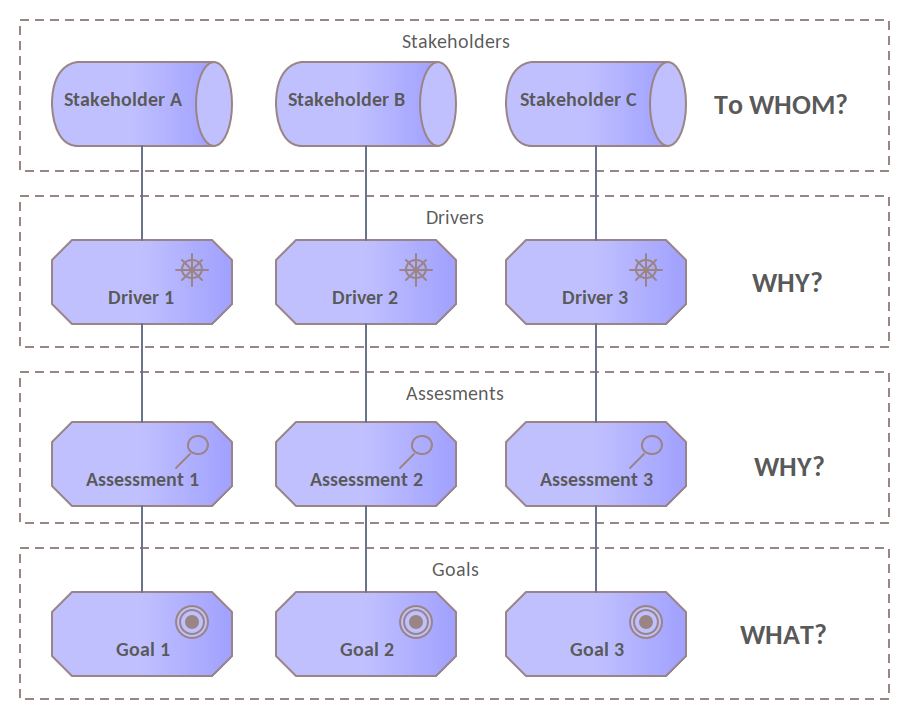
\includegraphics[width=0.7\textwidth]{images/views/Motivation view.png}
		\caption{The layered motivation structure}
		\label{fig:morivation-structure}
	\end{figure}
	
	\textit{Stakeholders} have associated interests, concerns or \textit{drivers}, which represent internal or external conditions that motivate an organisation to define goals.
	
	\textit{Assessments} represent results of analysis of the state of affairs with respect to a driver. They reveal strengths and weaknesses, opportunities and threats to an area of interest. Assessments are associated with \textit{goals} which represent a high-level statement of intent, plus direction to desired end state for an organisation and its stakeholders \citep{archimate3.1}. 
	
	In the context of the current project the following stakeholders have been identified:
	
	\enlargethispage{1em}
	
	\begin{itemize}
		\item OP legal analysis team (OP.C.2.003)
		\item Different OP services
		\item EU institutions
		\item LAM contractors
		\item Publications Office of the European Union (OP)
	\end{itemize}

	Next we present the motivation structure of spread over several sections addressing each stakeholder in part.
	
	\section{OP legal analysis team}

	The legal analysis team at the OP is the main stakeholder in this project. The main driver of this team is to establish a single point of access for the LAM data that can serve also as the single point of truth for this dataset. 
	
	\begin{figure}[h]
	\centering
	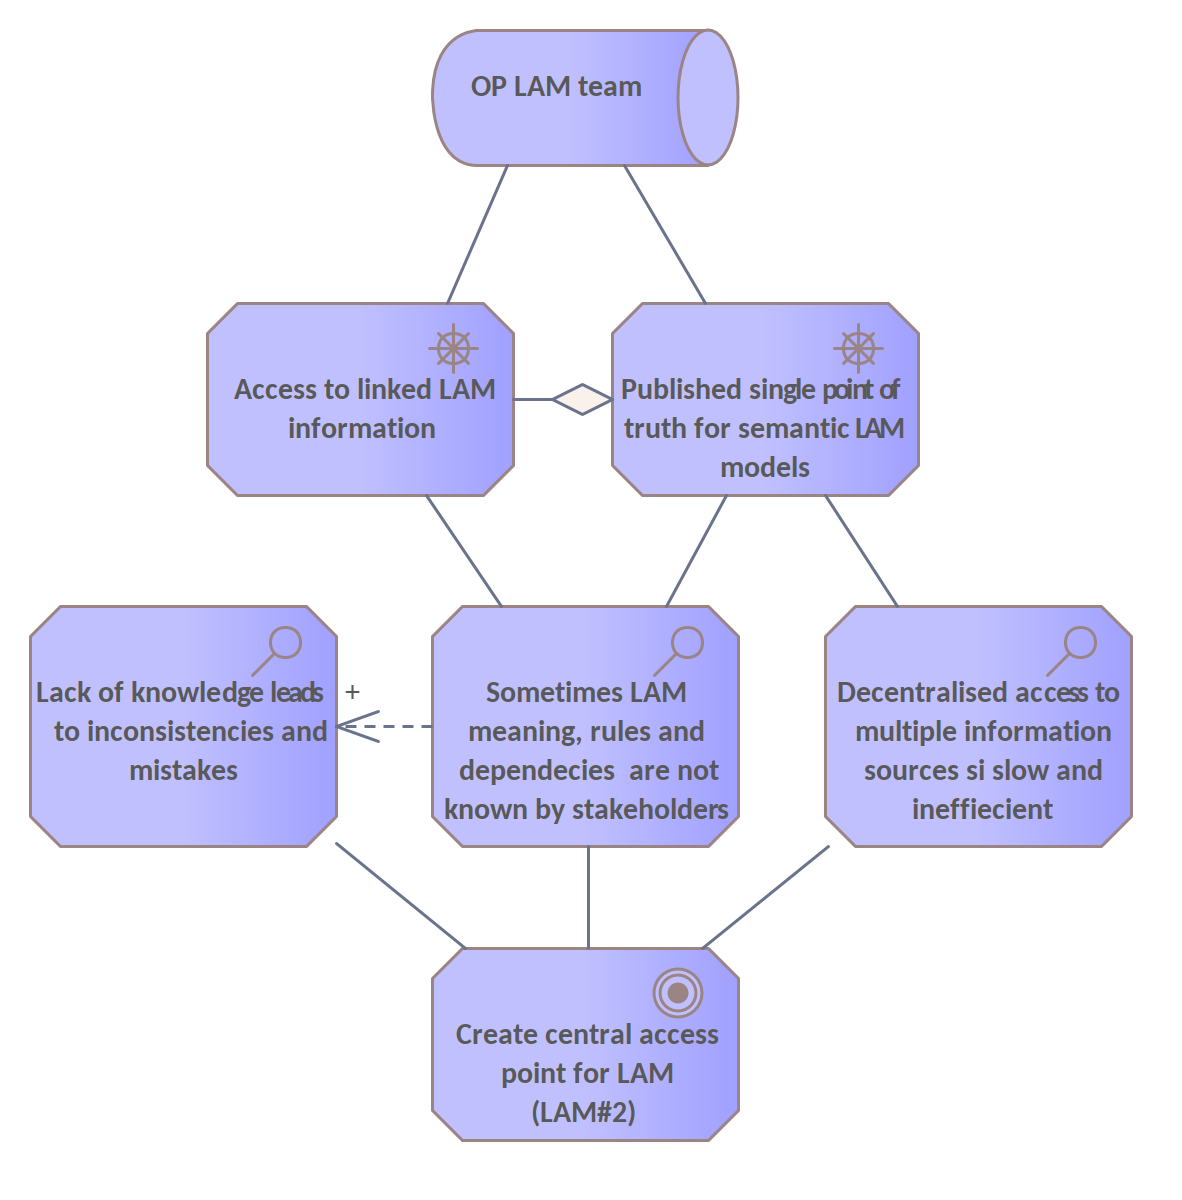
\includegraphics[width=0.67\textwidth]{images/motivation/LAM team motivation.png}
	\caption{Motivation structure of the OP legal analysis team}
	\label{fig:motivation-lam-team}
	\end{figure}
	
	One particular feature that is of special importance is to to also link other various datasets on which LAM relies, such as Common Data Model (CDM) \citep{cdm-francesconi2015ontology, cdm-francesconi2015semantic}, authority tables published at the EU Vocabularies\footnote{\url{https://op.europa.eu/en/web/eu-vocabularies}}, European Legislation Identifier (ELI) and others. The linked LAM information driver is a sub-goal to establishing a single point of access driver, and this is modelled via part-of relationship in \mbox{Figure \ref{fig:motivation-lam-team}}.
	
	In the context of the project these two drivers are hindered by three issues. First, multiple sources of information published in an uncoordinated manner on disparate sources are difficult to access and consume. This is especially the case when the information available at decentralised data sources needs to be used coherently in combination with other data sources.

	Another issue is that the meaning, rules and dependencies of the LAM model are sometimes not known by the stakeholders due to various reasons. One reason is the failure to find this information. Another reason is the informal explanation which may be incomplete, ambiguous or vague leading to multiple interpretations. And this leads to the third issue that the lack of precise formally defined knowledge is further propagated into the domain where LAM is applied and materialises as inconsistencies and mistakes in the data, system implementations, infrastructure configurations, exchange protocols and other aspects of the information systems. 
	
	To overcome these issues the goal of creating a central access point for the LAM data is adopted. This being the main goal of this project (LAM\#2). 	

	\section{Different OP services and EU institutions}
	
	At the Publications Office various internal units and the services they expose operate with legal data and metadata. Having access to the semantic description of the OP legal data is of primary concern for these services collectively. This is schematically depicted in Figure \ref{fig:motivation-op-services}.
	
	\begin{figure}[!th]
		\centering
		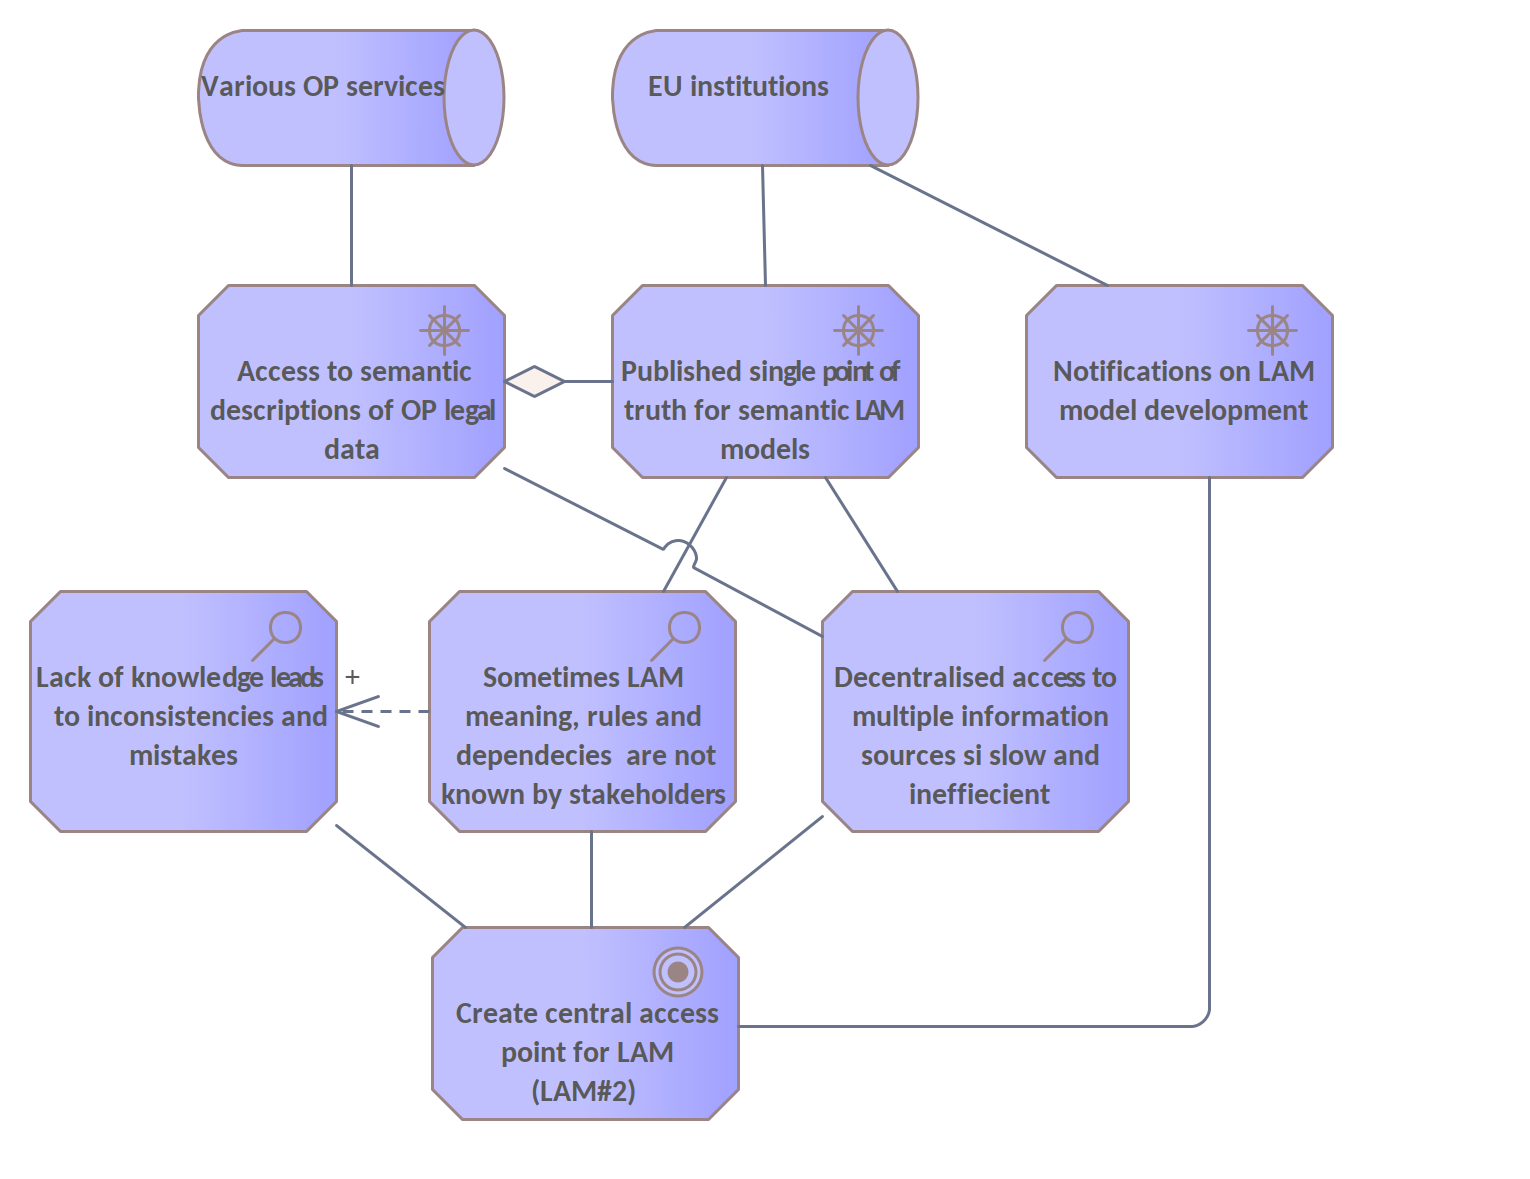
\includegraphics[width=0.789\textwidth]{images/motivation/EU institutions and OP services motivation.png}
		\caption{Motivation structure of different OP services}
		\label{fig:motivation-op-services}
	\end{figure}

	Implementation of the single point of access for semantic LAM model can be conceptualised as a sub-driver for the need to access semantic descriptions of OP legal data and metadata, which is represented through an aggregation relation in Figure \ref{fig:motivation-op-services}. Both motivations are hindered by the fact that decentralised access to multiple information sources is slow and inefficient. Moreover, LAM meaning, rules and dependencies are not always known to the interested stakeholders. To overcome these limitations, the current architecture aims at describing how a central dissemination point for LAM can be established. 
	
	The EU institutions, at large, as a collective consumer of legal metadata definitions has the same needs as the OP services. In addition, a notification mechanism is desired to inform the interested players of changes and updates in the LAM data. This need materialises directly as a feature of the system to disseminate LAM data. 
	
	\section{LAM contractors}

	The LAM contractors are a set of special stakeholders as they not only need to consult LAM data for information, but they are the agents that are actively involved in applying the specifications in practice. Often times, they will be those who inform the LAM team about possible issues in the LAM model or request extensions to it in order to accommodate new situations. The main driver for the LAM consultants is the consultancy on LAM and follow-up, depicted in Figure \ref{fig:motivation-lam-contractors}. 
		 	
	\begin{figure}[h]
		\centering
		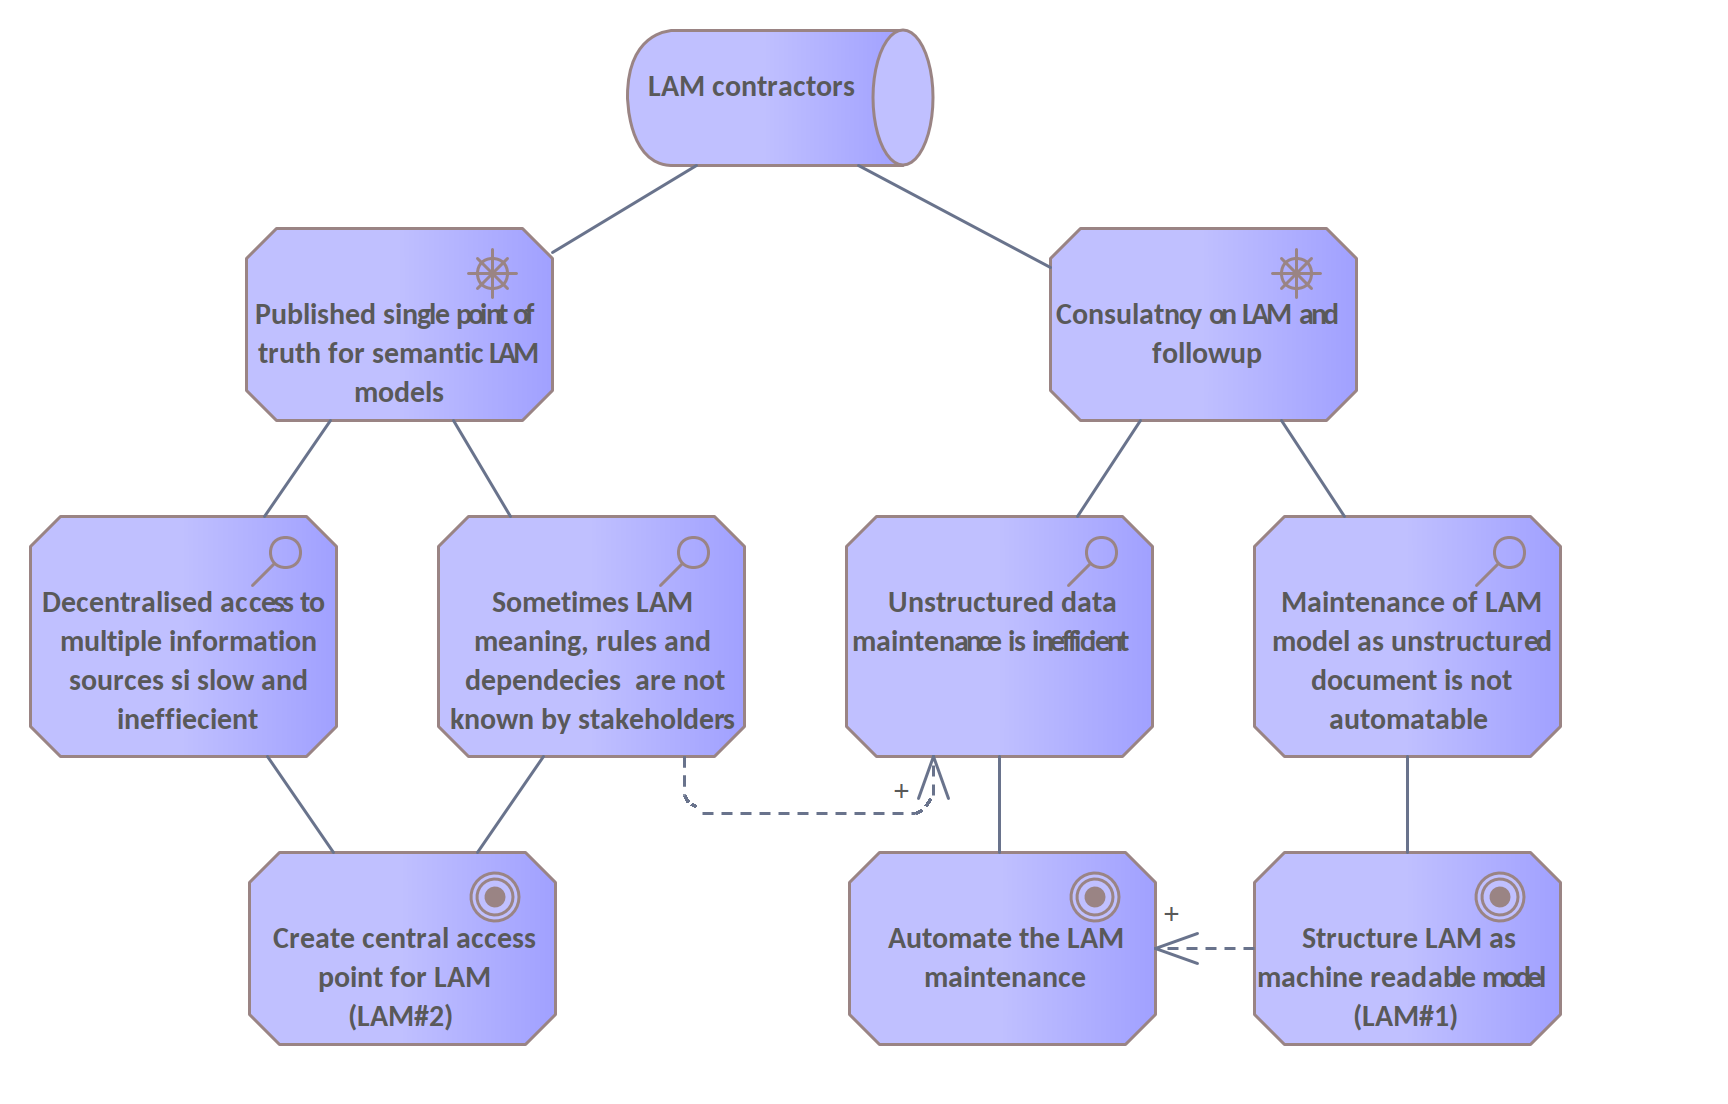
\includegraphics[width=0.95\textwidth]{images/motivation/LAM Contractors motivation.png}
		\caption{Motivation structure of LAM contractors}
		\label{fig:motivation-lam-contractors}
	\end{figure}

	Traditionally, the LAM model was maintained as a MS Word document that is an unstructured (at least not for the machines) data representation. A direct consequence of this approach is that no automation, validation or consistency checking is possible with such representations. To overcome this limitation an initiative to structure LAM data into a machine readable model was performed at the end of 2019 (referred as LAM\#1 project). LAM\#1 deliverables are available in the \textit{lam4vb3} GitHub repository\footnote{see \url{https://github.com/eu-vocabularies/lam4vb3}}.
		
	Another issue is that, as no machine assistance is possible to implement, the maintenance of these data becomes increasingly more difficult due to highly interlinked nature of the LAM model. This approach does not scale and is inefficient. 
	Moreover the effect is amplified as sometimes the LAM meaning, rules and dependencies are not known by the LAM contractors or even the LAM maintenance team. In order to overcome this limitation, a set of automation functionalities and processes shall be established. This automation is out of current project scope and shall be addressed elsewhere. 
	
	On the left side of Figure \ref{fig:motivation-lam-contractors}, the driver, assessments and goal are repeated from the sections above as they are central to the current project and are, therefore, shared by all of the stakeholders. 

	\section{Publications Office of the European Union}
	
	The Publications Office of the European Union defines drivers at a higher level of abstraction; yet they are very relevant to mention because the current project contributes directly to those interests. Figure \ref{fig:motivation-op} depicts the motivation structure of the OP relevant to the context of the current project. 
	
	OP is interested in the semantic operability both across EU institutions and the intra-institutional information systems. To increase the shared common conceptualisation captured by the data models, they need to carry a certain level of formality, semantics that shall be verifiable for completeness and especially for soundness. Unfortunately not all data is represented in machine readable format and even less is based on semantic models. 
	
	\begin{figure}[!h]
		\centering
		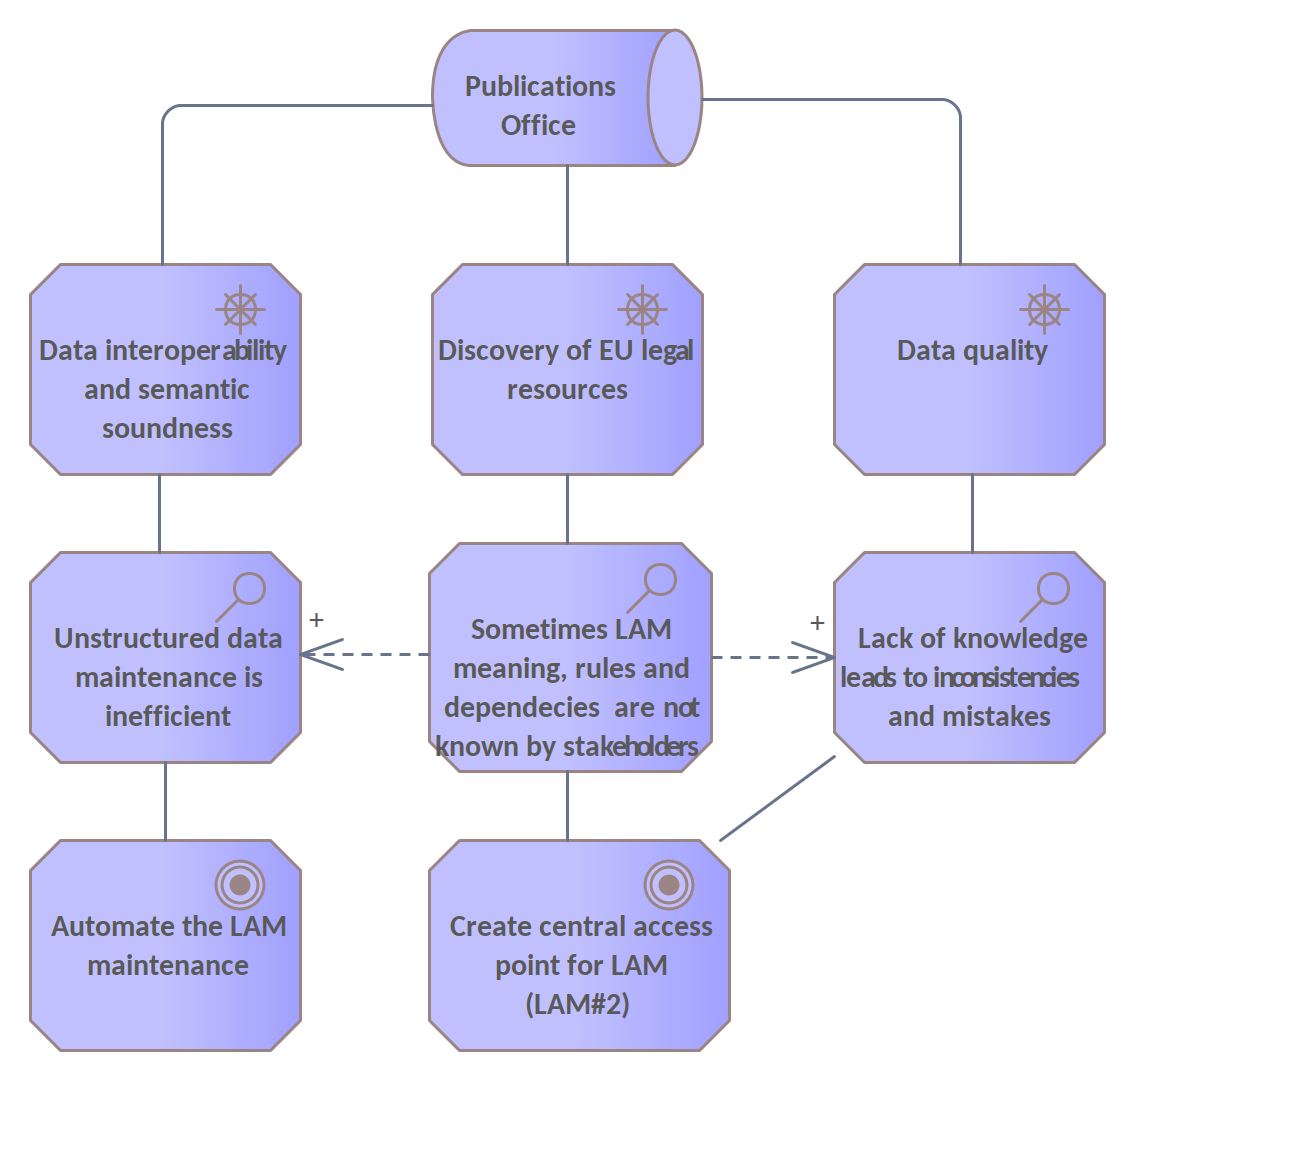
\includegraphics[width=0.859\textwidth]{images/motivation/OP level motivation (higher).png}
		\caption{Motivation structure of the Publications Office of the European Union}
		\label{fig:motivation-op}
	\end{figure}
	
	Another broad OP interest is maintaining and increasing by possible means the data quality. Causes such as lack of or impaired access to knowledge, unfortunately directly leads to inconsistencies and mistakes, which decrease the data quality. In order to overcome these limitations, the creation of a central access point for LAM addressed to a large extent the problem of knowledge shortage is required.
	
	Finally, a driver, which is at the heart of the OP as an institution, is to facilitate discovery of EU legal resources. In the context of the current project, this driver is hindered by the inability to easily find and access LAM meanings, rules and dependencies. Therefore, the dissemination of LAM data shall be done in such a way that the relations to external data sources are presented in an intuitive manner and the links are easy to navigate. Moreover, an inventory of links to the most used resources shall be disseminated with the LAM data. 
	